\documentclass[a4paper, 12pt]{article}%Tipagem
\usepackage[utf8]{inputenc}%Caracteres
\usepackage{svg, graphics, float}%Imagens
\usepackage[left=2cm,top=2cm,right=2cm,bottom=2cm]{geometry}%página
\usepackage{indentfirst, booktabs, setspace}%Formatação
\usepackage[portuges]{babel}%Idioma
\usepackage{fancyhdr} % Cabeçalho
\usepackage{csquotes}
\usepackage{amsmath, amssymb}

%Layout fofo
\pagestyle{fancy}
\fancyhead[L]{\Large{PME 5205}}
\fancyhead[C]{Controle Ótimo de Sistemas Dinâmicos}
\fancyhead[R]{{Mateus Silva Borges}}
\setlength{\headheight}{30pt}

\begin{document}
\onehalfspacing

\section*{Exame - 2026}

\subsection*{Questão 1}

\subsubsection*{Formulação do Problema}

O sistema dinâmico do oscilador harmônico (massa-mola) é descrito pela seguinte equação diferencial:
\begin{equation}
    \ddot{x}(t) + x(t) = u(t), \quad || u(t) || \le 1
\end{equation}

Definindo as variáveis de estado para o sistema:
\begin{align}
    x_1(t) &= x(t) \\
    x_2(t) &= \dot{x}(t)
\end{align}

Obtemos as equações de estado de primeira ordem:
\begin{align}
    \dot{x}_1(t) &= x_2(t) \\
    \dot{x}_2(t) &= -x_1(t) + u(t)
\end{align}

Na representação matricial $\dot{\mathbf{x}}(t) = \mathbf{A}\mathbf{x}(t) + \mathbf{B}u(t)$:
\begin{equation}
    \begin{bmatrix}
        \dot{x}_1 \\
        \dot{x}_2
    \end{bmatrix}
    =
    \begin{bmatrix}
        0 & 1 \\
        -1 & 0
    \end{bmatrix}
    \begin{bmatrix}
        x_1 \\
        x_2
    \end{bmatrix}
    +
    \begin{bmatrix}
        0 \\
        1
    \end{bmatrix} u
\end{equation}

As condições de contorno do problema para a transferência de estado até a origem são:
\begin{equation}
    \mathbf{x}(t_0) = \begin{bmatrix} a \\ b \end{bmatrix}, \quad \mathbf{x}(t_f) = \begin{bmatrix} 0 \\ 0 \end{bmatrix}
\end{equation}

Para o problema de tempo mínimo, o índice de performance a ser minimizado para um problema de Mayer é dado por:
\begin{equation}
    J = t_f
\end{equation}

\subsubsection*{Hamiltoniana e Equações Adjuntas}

A Hamiltoniana do problema de tempo mínimo com vínculos dinâmicos através dos multiplicadores adjuntos $\lambda_1$ e $\lambda_2$:

\begin{align}
    H &= \sum_{j=1}^{2} \lambda_j f_j = \lambda_1 x_2 + \lambda_2 (-x_1 + u) \\
    H &= -\lambda_2 x_1 + \lambda_1 x_2 + \lambda_2 u
\end{align}

As equações adjuntas dos co-estado são dadas:
\begin{align}
    \dot{\lambda}_1 &= -\frac{\partial H}{\partial x_1} = \lambda_2 \\
    \dot{\lambda}_2 &= -\frac{\partial H}{\partial x_2} = -\lambda_1
\end{align}

A partir do sistema linear adjunto, derivando a segunda equação e substituindo a primeira, obtém-se a dinâmica da função de chaveamento:
\begin{equation}
    \ddot{\lambda}_2 + \lambda_2 = 0
\end{equation}

A solução analítica de $\lambda_2$ é dada por:
\begin{equation}
    \lambda_2(t) = C_1 \sin(t + C_2)
\end{equation}

No entanto, a lei de controle para a otimização no interior da região permitida é dada por:
\begin{equation}
    \frac{\partial H}{\partial u} = 0 \implies \lambda_2(t) = 0
\end{equation}

Se $\lambda_2(t) = 0$, suas derivadas temporais também são nulas, implicando que $C_1 = 0$. Logo, o vetor adjunto é trivialmente nulo, o que é uma violação das condições necessárias para o Princípio de Máximo de Pontryagin, então não há solução ótima no interior da região permitida.

Portanto, a solução deve residir estritamente na fronteira da região permitida: $|| u(t) || = 1$.

\begin{align}
    u^*(t) &= \arg \underset{||u|| \le 1}{\max} H \\
    u^*(t) &= \arg \underset{||u|| \le 1}{\max} (\lambda_2 u(t)) \\
    u^*(t) &= \text{sign}(\lambda_2(t))
\end{align}

Para maximizar a Hamiltoniana em relação ao controle no intervalo restrito pela fronteira, o controle ótimo deve assumir o sinal da função de chaveamento $\lambda_2(t)$.

Como $\lambda_2(t)$ é uma senoide com frequência $\omega = 1$ rad/s, ela cruza o eixo do tempo mudando de sinal a cada $\pi$ segundos. Isso define um controle do tipo \textit{Bang-Bang}, onde o comando muda descontinuamente entre $+1$ e $-1$.

\subsubsection*{Lei de Controle Ótimo}

Se $u = +1$:
\begin{equation}
    \frac{dx_2}{dx_1} = \frac{\dot{x}_2}{\dot{x}_1} = \frac{-x_1 + 1}{x_2}
\end{equation}

Separando as variáveis e integrando:
\begin{equation}
    x_2 \, dx_2 + (x_1 - 1) \, dx_1 = 0 \implies (x_1 - 1)^2 + x_2^2 = R_+^2
\end{equation}

Analogamente, se $u = -1$:
\begin{equation}
    \frac{dx_2}{dx_1} = \frac{\dot{x}_2}{\dot{x}_1} = \frac{-x_1 - 1}{x_2}
\end{equation}

\begin{equation}
    (x_1 + 1)^2 + x_2^2 = R_-^2
\end{equation}

Conforme a Figura \ref{fig:chaveamento}, as trajetórias controladas são circunferências concêntricas, alternando entre os centros $(1, 0)$ e $(-1, 0)$. Para os demais pontos iniciais, o sistema evolui em arcos de circunferência até atingir o chaveamento principal.

\begin{figure}[H]
    \centering
    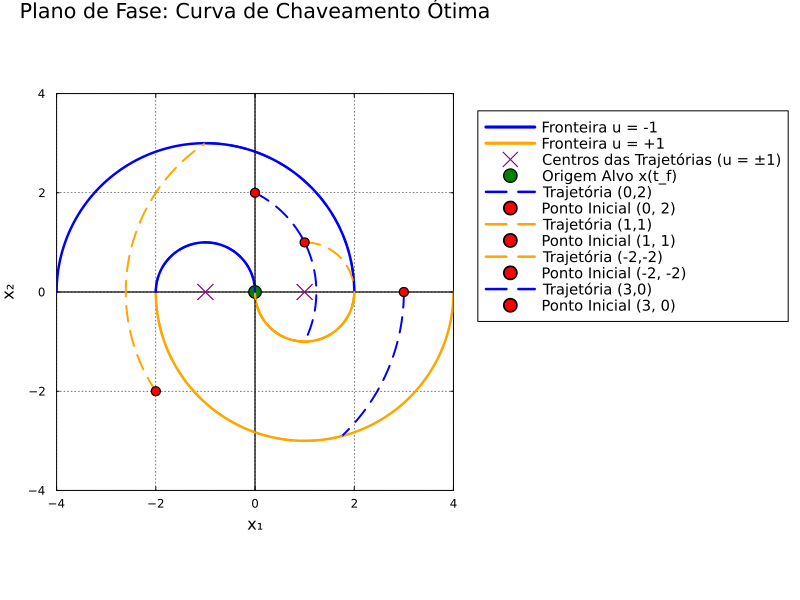
\includegraphics[width=0.8\textwidth]{img/chaveamentos_consolidados.png}
    \caption{Trajetórias de chaveamento do controle no plano de fases.}
    \label{fig:chaveamento}
\end{figure}

Para realizar a análise global no plano de fase, determina-se inicialmente se o ponto de partida encontra-se acima ou abaixo da curva de chaveamento ótima para definir o sentido do comando de força máxima . A partir daí, o estado do sistema percorre uma trajetória no sentido horário associada a esse controle até colidir com a fronteira de chaveamento . A cada interseção com essa curva, o comando inverte sua polaridade instantaneamente e o sistema passa a evoluir conforme o centro oposto, descrevendo arcos intermediários sequenciais . Esse comportamento cíclico conduz o corpo de qualquer quadrante ou distância até o trecho final de aproximação, onde a trajetória desliza diretamente até repousar na origem.

\newpage

\subsection*{Questão 2} 

\subsubsection*{Formulação do Problema}
O sistema dinâmico da planta de inércia é dado por:
\begin{equation}
    \ddot{x}(t) = u(t)
\end{equation}

Definindo as variáveis de estado:
\begin{align}
    x_1(t) &= x(t) \\
    x_2(t) &= \dot{x}(t)
\end{align}

Obtemos as equações de estado de primeira ordem:
\begin{align}
    \dot{x}_1(t) &= x_2(t) \\
    \dot{x}_2(t) &= u(t)
\end{align}

Para o problema de tempo mínimo, o índice de performance a ser minimizado para um problema de Lagrange é dado por:
\begin{equation}
    J = \int_{t_0}^{t_f} 1 \, dt
\end{equation}

Sujeito às seguintes restrições:
\begin{align}
    |u(t)| &\le 1 \\
    S(\mathbf{x}) = |x_2(t)| - 1 &\le 0
\end{align}

\subsubsection*{Hamiltoniana e Equações Adjuntas}
Quando a restrição de estado não está ativa, a Hamiltoniana é dada por:
\begin{equation}
    H = 1 + \lambda_1 x_2 + \lambda_2 u
\end{equation}

As equações adjuntas são:
\begin{align}
    \dot{\lambda}_1 &= -\frac{\partial H}{\partial x_1} = 0 \implies \lambda_1(t) = C_1 \\
    \dot{\lambda}_2 &= -\frac{\partial H}{\partial x_2} = - \lambda_1 \implies \lambda_2(t) = -C_1 t + C_2
\end{align}

Pelo Princípio do Máximo de Pontryagin, o controle ótimo que maximiza $H$ é:
\begin{equation}
u^*(t) = \text{sign}(\lambda_2(t)) = \pm 1
\end{equation}

As trajetórias no plano de fase são parábolas:
\begin{align}
    \text{Para } u = +1: \quad x_1 &= \frac{1}{2}x_2^2 + C_3 \\
    \text{Para } u = -1: \quad x_1 &= -\frac{1}{2}x_2^2 + C_4
\end{align}

Na fronteira do vínculo ($S = 0$), a trajetória deve satisfazer:
\begin{equation}
    \dot{S} = \dot{x}_2(t) = u(t) = 0
\end{equation}

Portanto, o controle na fronteira é $u^*(t) = 0$ e as trajetórias tornam-se linhas retas horizontais.

\subsubsection*{Lei de Controle Ótimo}
A curva de chaveamento primária $\Gamma$ é composta pelos arcos que levam diretamente à origem:
\begin{align}
\Gamma_+: \quad x_1 &= \frac{1}{2}x_2^2 \quad \text{para } -1 \le x_2 < 0 \\
\Gamma_-: \quad x_1 &= -\frac{1}{2}x_2^2 \quad \text{para } 0 < x_2 \le 1
\end{align}

A lei de controle em malha fechada é expressa como:
\begin{equation}
    u^*(x_1, x_2) =
    \begin{cases} 
    +1, & \text{se } x_1 < -\frac{1}{2}x_2|x_2| \text{ e } x_2 < 1 \\ 
    -1, & \text{se } x_1 > -\frac{1}{2}x_2|x_2| \text{ e } x_2 > -1 \\
    0, & \text{se } (x_2 = 1 \text{ e } x_1 < -0.5) \text{ ou } (x_2 = -1 \text{ e } x_1 > 0.5) 
    \end{cases}
\end{equation}

A lei de controle é representada graficamente na Figura \ref{fig:parabolas}:

\begin{figure}[H]
    \centering
    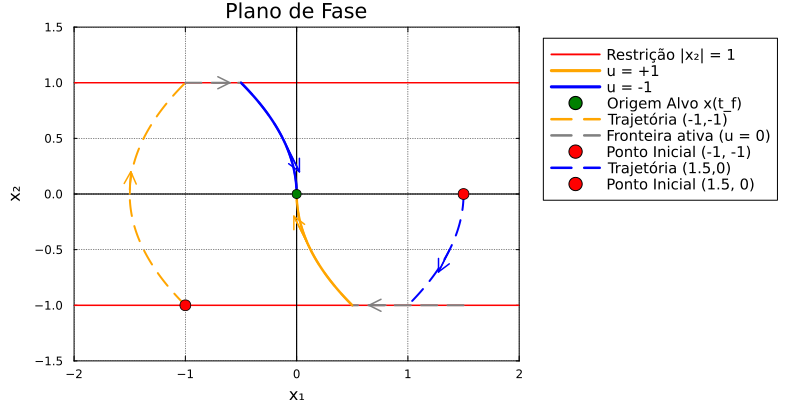
\includegraphics[width=0.9\textwidth]{img/trajetorias_parabolicas.png}
    \caption{Trajetórias de chaveamento do controle no plano de fases para a planta de inércia.}
    \label{fig:parabolas}
\end{figure}

\newpage
 
\subsection*{Questão 3} 

O modelo físico considerado é representado na Figura \ref{fig:circuito}.

\begin{figure}[H]
    \centering
    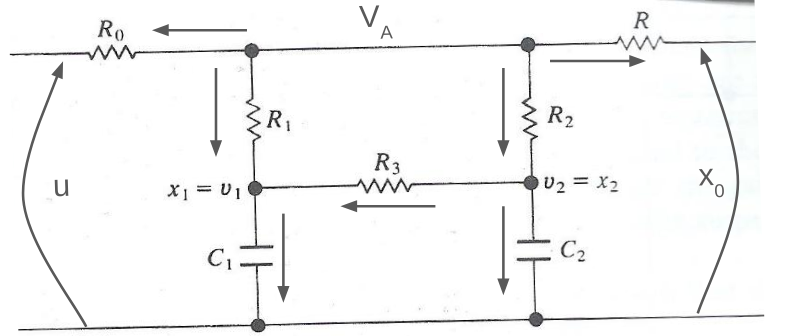
\includegraphics[width=0.8\textwidth]{img/circuito.png}
    \caption{Circuito elétrico para o controle de temperatura. As setas curvas de tensão indicam a entrada de controle $u$, que representa o aquecedor, e a entrada de distúrbio $x_0$, que representa o ambiente externo. As setas ao longo do circuito representam a convenção das correntes elétricas.}
    \label{fig:circuito}
\end{figure}

\subsubsection*{a)}

Aplicando a Lei das Correntes de Kirchhoff para o nó de $v_A$:
\begin{equation}
    \frac{v_A - u}{R_0} + \frac{v_A - v_1}{R_1} + \frac{v_A - v_2}{R_2} + \frac{v_A - x_0}{R} = 0
\end{equation}

Analogamente para o nó de $x_1$:
\begin{equation}
    \frac{v_A - v_1}{R_1} + \frac{v_2 - v_1}{R_3} = C_1 \frac{dv_1}{dt}
\end{equation}

Analogamente para o nó de $x_2$:
\begin{equation}
    \frac{v_A - v_2}{R_2} = \frac{v_2 - v_1}{R_3} + C_2 \frac{dv_2}{dt}
\end{equation}

Por simplicidade, definimos as condutâncias elétricas:
\begin{align*}
    G_0 = \frac{1}{R_0}, \quad G_1 = \frac{1}{R_1}, \quad G_2 = \frac{1}{R_2}, \quad G_3 = \frac{1}{R_3}, \quad G = \frac{1}{R}
\end{align*}
\begin{equation*}
    \Sigma G = G_0 + G_1 + G_2 + G
\end{equation*}

Dessa forma, a tensão no nó $v_A$ é expressa como:
\begin{equation}
    v_A = \frac{G_1 x_1 + G_2 x_2 + G_0 u + G x_0}{\Sigma G}
\end{equation}

Substituindo na representação canônica linear $\dot{\mathbf{x}}(t) = \mathbf{A}\mathbf{x}(t) + \mathbf{B}u(t) + \mathbf{E}x_0(t)$, obtemos:
\begin{equation}
    \begin{bmatrix} 
        \dot{x}_1 \\ 
        \dot{x}_2 
    \end{bmatrix} = 
    \begin{bmatrix} 
        \frac{1}{C_1}\left(\frac{G_1^2}{\Sigma G} - G_1 - G_3\right) & \frac{1}{C_1}\left(\frac{G_1 G_2}{\Sigma G} + G_3\right) \\ 
        \frac{1}{C_2}\left(\frac{G_1 G_2}{\Sigma G} + G_3\right) & \frac{1}{C_2}\left(\frac{G_2^2}{\Sigma G} - G_2 - G_3\right) 
    \end{bmatrix} 
    \begin{bmatrix} 
        x_1 \\ 
        x_2 
    \end{bmatrix} + 
    \begin{bmatrix} 
        \frac{G_1 G_0}{C_1 \Sigma G} \\ 
        \frac{G_2 G_0}{C_2 \Sigma G} 
    \end{bmatrix} u + 
    \begin{bmatrix} 
        \frac{G_1 G}{C_1 \Sigma G} \\ 
        \frac{G_2 G}{C_2 \Sigma G} 
    \end{bmatrix} x_0
\end{equation}

\subsubsection*{b)}

O modelo dinâmico linear é representado pelas equações diferenciais:
\begin{align*}
\dot{x}_1 &= -x_1 + x_2 + u \\
\dot{x}_2 &= x_1 - 3x_2 + 2x_0
\end{align*}

\subsubsection*{c)}

Para determinar se o sistema permite o controle de qualquer variável de estado ou de uma combinação delas, analisamos a sua controlabilidade com base na teoria de sistemas lineares. Desconsideramos a entrada de perturbação externa $x_0$ para a análise de controlabilidade, uma vez que sinais exógenos não alteram as propriedades intrínsecas de controle do par dinâmico. Logo, escrevemos o sistema na forma matricial padrão $\dot{x} = Ax + Bu$:
\begin{equation}
A = \begin{bmatrix} -1 & 1 \\ 1 & -3 \end{bmatrix}, \quad B = \begin{bmatrix} 1 \\ 0 \end{bmatrix}
\end{equation}

Para um sistema de segunda ordem ($n=2$), a matriz de controlabilidade é dada por:
\begin{equation}
\begin{bmatrix} B & AB \end{bmatrix}
\end{equation}

Calculando o produto matricial $AB$:
\begin{equation}
AB = \begin{bmatrix} -1 & 1 \\ 1 & -3 \end{bmatrix} \begin{bmatrix} 1 \\ 0 \end{bmatrix} = \begin{bmatrix} -1 \\ 1 \end{bmatrix}
\end{equation}

Montando a matriz de controlabilidade:
\begin{equation}
\begin{bmatrix} 1 & -1 \\ 0 & 1 \end{bmatrix}
\end{equation}
A matriz de controlabilidade possui posto completo ($\text{rank} = 2$), indicando que o sistema é completamente controlável, logo, é matematicamente possível transferir o sistema de qualquer estado inicial para qualquer outro estado final em tempo finito. 

No entanto, como o sistema possui apenas uma única entrada de controle independente, ele apresenta apenas um grau de liberdade de atuação. Consequentemente, não é possível fazer com que as duas variáveis de estado ($x_1$ e $x_2$) sigam, de forma independente e simultânea, duas trajetórias arbitrárias quaisquer. O problema só permite o controle efetivo e independente de uma das variáveis de estado ou de uma combinação linear específica delas como, por exemplo, a saída ponderada $y = c_1x_1 + c_2x_2$).

\subsubsection*{d)}

Alinhando o problema com a formulação padrão do Controlador Linear Quadrático (LQ) apresentada nas notas de aula, definimos o sistema dinâmico linear homogêneo desconsiderando a perturbação constante $x_0$ na matriz de entrada:

\begin{equation}
\dot{\mathbf{x}}(t) = A\mathbf{x}(t) + B u(t)
\end{equation}

Onde as matrizes do sistema são dadas por:
\begin{equation}
A = \begin{bmatrix} -1 & 1 \\ 1 & -3 \end{bmatrix}, \quad B = \begin{bmatrix} 1 \\ 0 \end{bmatrix}
\end{equation}

O Índice de Performance ($IP$) a ser minimizado no intervalo $[0, T]$ é dado por:
\begin{equation}
IP = \int_0^T \left[ (c_1x_1 + c_2x_2)^2 + k^2u^2 \right] dt
\end{equation}

Para expressá-lo na forma quadrática padrão das notas de aula, multiplicamos o índice por $\frac{1}{2}$:
\begin{equation}
\bar{IP} = \frac{1}{2} \int_0^T \left[ \mathbf{x}^T W_1 \mathbf{x} + 2\mathbf{x}^T W_2 u + u^T W_3 u \right] dt
\end{equation}

Comparando as duas expressões, obtemos:
\begin{equation}
W_1 = \begin{bmatrix} 2c_1^2 & 2c_1c_2 \\ 2c_1c_2 & 2c_2^2 \end{bmatrix}, \quad W_2 = \begin{bmatrix} 0 \\ 0 \end{bmatrix}, \quad W_3 = 2k^2
\end{equation}
Como não há penalização explícita do estado final, a matriz de custo terminal é nula:
\begin{equation}
\bar{Q}_f = \begin{bmatrix} 0 & 0 \\ 0 & 0 \end{bmatrix}
\end{equation}


A evolução temporal da matriz $P(t) = \begin{bmatrix} p_1(t) & p_2(t) \\ p_2(t) & p_3(t) \end{bmatrix}$ é governada pela Equação Diferencial de Riccati:
\begin{equation}
\dot{P} = -PA - A^TP - W_1 + P B W_3^{-1} B^T P
\end{equation}

Substituindo as matrizes $A$, $B$, $W_1$ e $W_3$, calculamos os blocos da equação:
\begin{align*}
-PA - A^TP &= \begin{bmatrix} 2(p_1 - p_2) & -p_1 + 4p_2 - p_3 \\ -p_1 + 4p_2 - p_3 & 2(-p_2 + 3p_3) \end{bmatrix} \\
P B W_3^{-1} B^T P &= \begin{bmatrix} p_1 \\ p_2 \end{bmatrix} \frac{1}{2k^2} \begin{bmatrix} p_1 & p_2 \end{bmatrix} = \frac{1}{2k^2} \begin{bmatrix} p_1^2 & p_1p_2 \\ p_1p_2 & p_2^2 \end{bmatrix}
\end{align*}

Desta forma, obtemos o sistema de equações diferenciais ordinárias não-lineares acopladas para os elementos de $P(t)$:
\begin{align*}
\dot{p}_1(t) &= 2\big(p_1(t) - p_2(t)\big) - 2c_1^2 + \frac{p_1^2(t)}{2k^2} \\
\dot{p}_2(t) &= -p_1(t) + 4p_2(t) - p_3(t) - 2c_1c_2 + \frac{p_1(t)p_2(t)}{2k^2} \\
\dot{p}_3(t) &= 2\big(-p_2(t) + 3p_3(t)\big) - 2c_2^2 + \frac{p_2^2(t)}{2k^2}
\end{align*}

Como $\bar{Q}_f = 0$, a integração deve ser realizada de trás para frente no tempo (do instante $t = T$ até $t = 0$) a partir de:
\begin{equation}
p_1(T) = 0, \quad p_2(T) = 0, \quad p_3(T) = 0
\end{equation}


A lei de controle ótima em malha fechada é determinada a partir da relação estado-coestado:
\begin{equation}
u^*(\mathbf{x},t) = -W_3^{-1} B^T P(t) \mathbf{x}(t)
\end{equation}

Substituindo os valores correspondentes:
\begin{equation}
u^*(\mathbf{x},t) = -\frac{1}{2k^2} \begin{bmatrix} 1 & 0 \end{bmatrix} \begin{bmatrix} p_1(t) & p_2(t) \\ p_2(t) & p_3(t) \end{bmatrix} \begin{bmatrix} x_1(t) \\ x_2(t) \end{bmatrix}
\end{equation}

\begin{equation}
\mathbf{u^*(\mathbf{x},t) = -\frac{1}{2k^2} \big[ p_1(t)x_1(t) + p_2(t)x_2(t) \big]}
\end{equation}

\subsubsection*{e)}

Substituindo os valores numéricos fornecidos ($k=1, c_1=1, c_2=1$), as matrizes de ponderação são:
\begin{equation}
A = \begin{bmatrix} -1 & 1 \\ 1 & -3 \end{bmatrix}, \quad B = \begin{bmatrix} 1 \\ 0 \end{bmatrix}, \quad Q = \begin{bmatrix} 1 & 1 \\ 1 & 1 \end{bmatrix}, \quad R = 1
\end{equation}

Definindo a matriz simétrica e definida positiva $P$ como:
\begin{equation}
P = \begin{bmatrix} p_1 & p_2 \\ p_2 & p_3 \end{bmatrix}
\end{equation}

Substituindo os blocos de volta na equação de Riccati, obtemos três equações escalares acopladas:
\begin{align*}
\text{Elemento } (1,1): \quad & -2p_1 + 2p_2 - p_1^2 + 1 = 0 \implies 2p_2 = p_1^2 + 2p_1 - 1 \quad \text{(Eq. 1)} \\
\text{Elemento } (2,2): \quad & 2p_2 - 6p_3 - p_2^2 + 1 = 0 \implies 6p_3 = 2p_2 - p_2^2 + 1 \quad \text{(Eq. 2)} \\
\text{Elemento } (1,2): \quad & p_1 - 4p_2 + p_3 - p_1p_2 + 1 = 0 \quad \text{(Eq. 3)}
\end{align*}

A única raiz real e positiva que garante uma matriz $P$ definida positiva é dada exatamente por:
\begin{equation}
p_1 = -4 + \sqrt{13 + 4\sqrt{5}} \approx 0,6845
\end{equation}

Substituindo este valor de volta na relação do Elemento (1,1) para encontrar $p_2$:
\begin{equation}
p_2 = \frac{(0,6845)^2 + 2(0,6845) - 1}{2} \approx 0,4187
\end{equation}

A lei de controle por realimentação linear de estados é expressa por:
\begin{equation}
u^*(\mathbf{x}) = -R^{-1}B^T P \mathbf{x}(t) = -\begin{bmatrix} 1 & 0 \end{bmatrix} \begin{bmatrix} p_1 & p_2 \\ p_2 & p_3 \end{bmatrix} \begin{bmatrix} x_1(t) \\ x_2(t) \end{bmatrix}
\end{equation}
\begin{equation}
u^*(\mathbf{x}) = -p_1x_1(t) - p_2x_2(t)
\end{equation}

Substituindo os valores calculados de $p_1$ e $p_2$, a lei de realimentação fechada é:
\begin{equation}
\mathbf{u^*(t) \approx -0,6845 \, x_1(t) - 0,4187 \, x_2(t)}
\end{equation}

\newpage

\subsection*{Questão 4}

\subsubsection*{Formulação do Problema}

As equações de movimento são dadas por: 
\begin{align}
    \dot{x}(t) &= V \cos\theta(t) + u \\
    \dot{y}(t) &= V \sin\theta(t)
\end{align}

Onde a variável de controle é dada pelo ângulo de guinada $\theta$. O índice de desempenho a ser maximizado é definido pela área:
\begin{equation}
    A = \oint y \, dx = \int_{0}^{T} y(t) \dot{x}(t) \, dt = \int_{0}^{T} y (V \cos\theta + u) \, dt
\end{equation}

\subsubsection*{Hamiltoniana e Equações Adjuntas}

Utilizando a formulação do Princípio do Máximo de Pontryagin, construímos a função Hamiltoniana $H$:
\begin{equation}
    H = L + \lambda_1 \dot{x} + \lambda_2 \dot{y}
\end{equation}
\begin{equation}
    H = y(V \cos\theta + u) + \lambda_1 (V \cos\theta + u) + \lambda_2 (V \sin\theta)
\end{equation}

Agrupando os termos comuns associados à velocidade do ar $V$ e do vento $u$, a Hamiltoniana assume a forma compacta:
\begin{equation}
    H = (y + \lambda_1)(V \cos\theta + u) + \lambda_2 V \sin\theta
\end{equation}

As equações adjuntas são dadas por:
\begin{align}
    \dot{\lambda}_1(t) &= -\frac{\partial H}{\partial x} = 0 \implies \lambda_1(t) = C_1 \quad (\text{constante}) \\
    \dot{\lambda}_2(t) &= -\frac{\partial H}{\partial y} = -(V \cos\theta + u) = -\dot{x}(t) \implies \lambda_2(t) = -x(t) + C_2
\end{align}

\subsubsection*{Lei de Controle Ótimo}
O ângulo de guinada ótimo $\theta^*(t)$ que maximiza a Hamiltoniana é dado por:
\begin{equation}
    \frac{\partial H}{\partial \theta} = (y + C_1)(-V \sin\theta) + (-x + C_2)(V \cos\theta) = 0
\end{equation}

Dividindo a expressão pela constante de velocidade $V$, isolamos a lei de tangência ótima para a orientação da aeronave:
\begin{equation}
    \tan\theta = \frac{-x + C_2}{y + C_1}
\end{equation}

\subsubsection*{Análise Geométrica}
Transladando o sistema de coordenadas para simplificar a análise geométrica:
\begin{align}
    X &= x - C_2 \\
    Y &= y + C_1
\end{align}

Logo, a análise reduz-se a $\tan\theta = -\frac{X}{Y}$:
\begin{equation}
    \cos\theta = \frac{Y}{\sqrt{X^2 + Y^2}}, \quad \sin\theta = \frac{-X}{\sqrt{X^2 + Y^2}}
\end{equation}

Analisando diretamente o comportamento geométrico:
\begin{equation}
    \frac{dX}{dY} = \frac{\dot{X}}{\dot{Y}} = \frac{\frac{V Y}{\sqrt{X^2 + Y^2}} + u}{\frac{-V X}{\sqrt{X^2 + Y^2}}} = -\frac{Y}{X} - \frac{u}{V}\frac{\sqrt{X^2 + Y^2}}{X}
\end{equation}

Multiplicando os dois lados por $X \, dY$:
\begin{equation}
    X \, dX + Y \, dY = -\frac{u}{V}\sqrt{X^2 + Y^2} \, dY
\end{equation}

Aplicando a transformação para coordenadas radiais:
\begin{equation}
    R^2 = X^2 + Y^2 \implies R \, dR = X \, dX + Y \, dY
\end{equation}

Integrando ambos os lados em relação a uma constante de integração radial $R_0$:
\begin{align}
    X \, dX + Y \, dY &= -\frac{u}{V}\sqrt{X^2 + Y^2} \, dY \\
    R dR &= -\frac{u}{V} R dY \\ 
    \int dR &= \int -\frac{u}{V} dY \\
    R - R_0 &= -\frac{u}{V} Y \\
    R^2 &= \left(R_0 - \frac{u}{V}Y\right)^2 \\
    X^2 + Y^2 &= \left(R_0 - \frac{u}{V}Y\right)^2 \\
    X^2 + Y^2 &= R_0^2 - 2R_0\frac{u}{V}Y + \frac{u^2}{V^2}Y^2 \\
    X^2 + Y^2\left(1 - \frac{u^2}{V^2}\right) + 2R_0\frac{u}{V}Y &= R_0^2
\end{align}

Completando o quadrado perfeito em $Y$, conseguimos ajustar a equação para a forma padrão de uma elipse:
\begin{equation}
    \frac{X^2}{\frac{R_0^2}{1 - \frac{u^2}{V^2}}} + \frac{\left(Y + \frac{R_0 u/V}{1 - \frac{u^2}{V^2}}\right)^2}{\frac{R_0^2}{\left(1 - \frac{u^2}{V^2}\right)^2}} = 1
\end{equation}

\begin{itemize}
    \item Na ausência de vento ($u = 0$), a equação se torna a equação de uma circunferência $X^2 + Y^2 = R_0^2$
    \item Considerando a velocidade do vento $u$, a curva de espera ótima deforma-se em uma elipse cujo centro sofre um deslocamento ortogonal à direção do vento e cujos eixos guardam a proporção exata da excentricidade
    \begin{equation}
        \frac{\text{Semieixo horizontal } (x)}{\text{Semieixo vertical } (y)} = \sqrt{1 - \frac{u^2}{V^2}}
    \end{equation}
\end{itemize}

\newpage

\subsection*{Questão 5}

\subsubsection*{Algoritmo Genético}

O Algoritmo Genético (GA) é um método meta-heurístico de otimização global baseado nos princípios da seleção natural e da genética biológica. Ao contrário dos métodos determinísticos baseados em gradientes, o GA opera sobre uma população de indivíduos simultâneos tornando-se altamente robusto contra mínimos locais em superfícies de custo não-convexas ou descontínuas.

O vetor de variáveis de decisão representa o genótipo do indivíduo, enquanto os valores calculados de massa, tensão de pico e energia compõem o fenótipo avaliado pelo operador de aptidão (fitness). Esse método de otimização de grau zero representa um balanço ótimo entre exploração (mapeamento global) e explotação (refinamento local). Esse equilíbrio dinâmico pode ser calibrado para uma melhor convergência através da escolha dos mecanismos e operadores genéticos.

\begin{itemize}
    \item \textbf{Seleção por Torneio (\texttt{TournamentSelection(K=3, N=50)}):} O tamanho da população é fixado em $N=50$ indivíduos. Para cada vaga de reprodução, $K=3$ indivíduos são amostrados aleatoriamente e o de melhor aptidão (considerando a função objetivo e as penalidades de restrição) é selecionado como pai. Definir $K=3$ estabelece uma pressão seletiva calibrada: mitiga a convergência prematura nas gerações iniciais mantendo a diversidade genética, mas garante que os genes mais aptos guiem a busca.
    \item \textbf{Crossover Uniforme (\texttt{UniformCrossover(p=0.80)}):} Com uma probabilidade de $80\%$, os pais selecionados trocam material genético. No crossover uniforme, cada gene (coordenada do vetor de decisão) do descendente é escolhido de forma independente a partir de um dos genitores com base em uma distribuição equilibrada. Esse operador possui alto poder exploratório e destrói correlações posicionais rígidas, permitindo combinar de forma eficiente parâmetros geométricos ($d, h$) e operacionais ($\omega$).
    \item \textbf{Mutação Polinomial (\texttt{PolynomialMutation}):} Essencial para codificação real, gera perturbações contínuas baseadas em uma distribuição polinomial em torno do valor original do gene. Os valores adotados para esse operador são adaptados à dimensão do problema e à natureza das restrições:
    \begin{itemize}
        \item \textbf{Problema I (Dimensão 2):} Adota-se um índice de distribuição $\eta=5$ e probabilidade $p_m=1/2$. Um valor menor de $\eta$ abre a curva de probabilidade, permitindo mutações com saltos mais amplos para explorar de forma agressiva o plano bidimensional.
        \item \textbf{Problema II (Dimensão 3):} Utiliza-se $\eta=10$ e probabilidade reduzida $p_m=1/3$. Aumentar o índice estreita a curva de mutação, gerando perturbações menores, predominantemente locais. Como o espaço tridimensional é maior e restrições centrífugas são severas, saltos longos gerariam muitos indivíduos inviáveis, justificando um refinamento mais suave ao longo das restrições.
    \end{itemize}
    \item \textbf{Seleção Ambiental Elitista (\texttt{ElitistReplacement}):} Aplica uma estratégia onde os $N=50$ melhores indivíduos da população conjunta de pais e filhos são preservados para a geração subsequente. Isso assegura que a melhor solução de energia mecânica encontrada nunca sofra regressão ao longo do horizonte evolutivo, garantindo convergência monotônica.
\end{itemize}


No contexto do projeto do volante de inércia (KERS), o objetivo é maximizar a energia cinética armazenada, mapeada como um problema de minimização do valor negativo dessa energia para alinhar com a arquitetura das bibliotecas de programação adotadas. 

\subsubsection*{Velocidade Angular Fixa (Problema I)}

A topologia do espaço de busca bidimensional do Problema I, onde a velocidade angular é fixada na rotação nominal de $3000$ rpm, foi graficamente mapeada a partir da função objetivo. A Figura~\ref{fig:contorno} apresenta as curvas de nível da energia armazenada calculada negativamente para fins de minimização algorítmica, variando em função do diâmetro $d$ e da altura $h$ do disco de aço.

\begin{figure}[H]
    \centering
    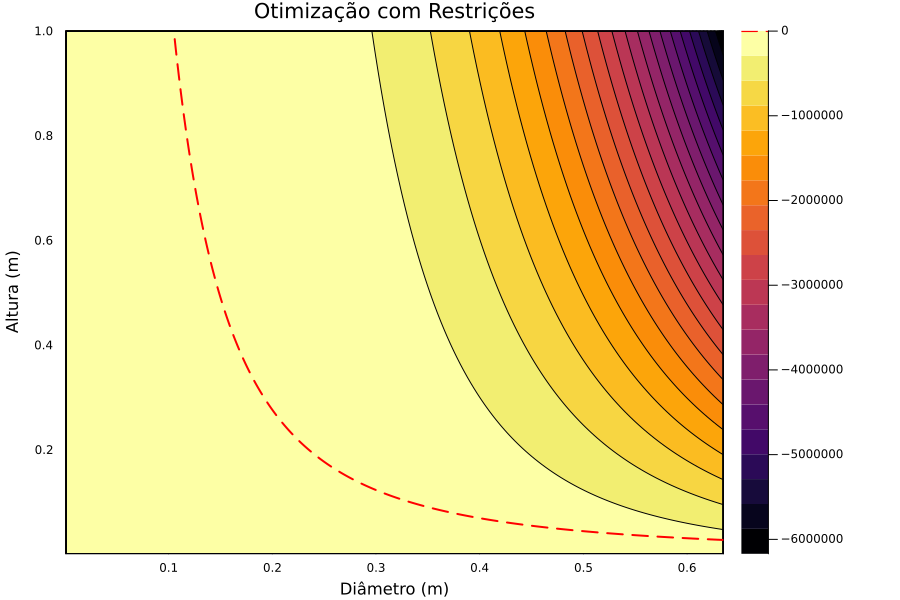
\includegraphics[width=0.6\textwidth]{img/problema_1_contorno.png}
    \caption{Representação gráfica do contorno da função objetivo do problema 1 de velocidade angular fixa em $3000$ rpm. A linha tracejada representa a fronteira de estados admissíveis quanto à restrição de massa.}
    \label{fig:contorno}
\end{figure}

A análise das curvas de nível da Figura~\ref{fig:contorno} demonstra que a restrição de tensão e restrição de massa delimitam rigidamente o diâmetro máximo admissível. A equação de tensão centrífuga de pico independe da espessura ou altura $h$, essa barreira se comporta como uma reta vertical estrita paralela ao eixo das ordenadas. Paralelamente, a restrição de massa máxima estabelece uma fronteira hiperbólica regida pela equação geométrica. O ponto ótimo global determinado pelo GA localiza-se exatamente no vértice de interseção entre a restrição hiperbólica de massa ativa e o limite geométrico de diâmetro, onde as duas restrições de desigualdade se tornam ativas simultaneamente.

O monitoramento do desempenho computacional e da taxa de aprendizado do algoritmo genético é feito pelo gráfico de convergência do funcional. A Figura \ref{fig:convergencia_1} ilustra a evolução temporal do melhor valor da função objetivo em relação ao número acumulado de chamadas da função objetivo no interior do loop adaptativo.

\begin{figure}[H]
    \centering
    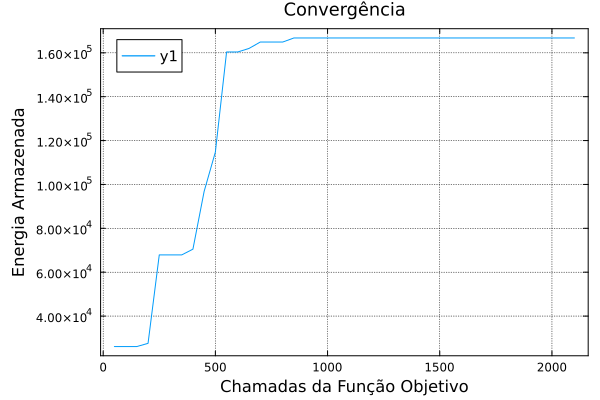
\includegraphics[width=0.6\textwidth]{img/problema_1_convergencia.png}
    \caption{Convergência da função objetivo do problema 1 de velocidade angular fixa em $3000$ rpm.}
    \label{fig:convergencia_1}
\end{figure}

O perfil gráfico obtido na Figura \ref{fig:convergencia_1} evidencia degraus evolutivos muito claros, comportamento típico de mecanismos de substituição ambiental elitista. Os longos patamares horizontais representam períodos em que a população consolida sua diversidade local ou elimina candidatos inviáveis sem alterações no melhor indivíduo absoluto, enquanto os saltos verticais abruptos indicam a descoberta de novos candidatos ótimos via mutação ou recombinação (crossover) uniforme bem-sucedida. A estabilização completa ocorre rapidamente, atingindo o patamar assintótico estável de aproximadamente $1,60 \times 10^5$ J por volta de apenas 1000 chamadas à função objetivo.

A dinâmica de movimentação e a transição entre as fases de exploração global e explotação local podem ser visualizadas por meio da distribuição espacial dos indivíduos no plano $(d, h)$. A Figura \ref{fig:populacao_1} decompõe essa evolução populacional em momentos-chave da execução do algoritmo, retratando as Gerações 1, 2, 3, 4, 6, 21 e 42 para evidenciar o estreitamento estocástico populacional .

\begin{figure}[H]
    \centering
    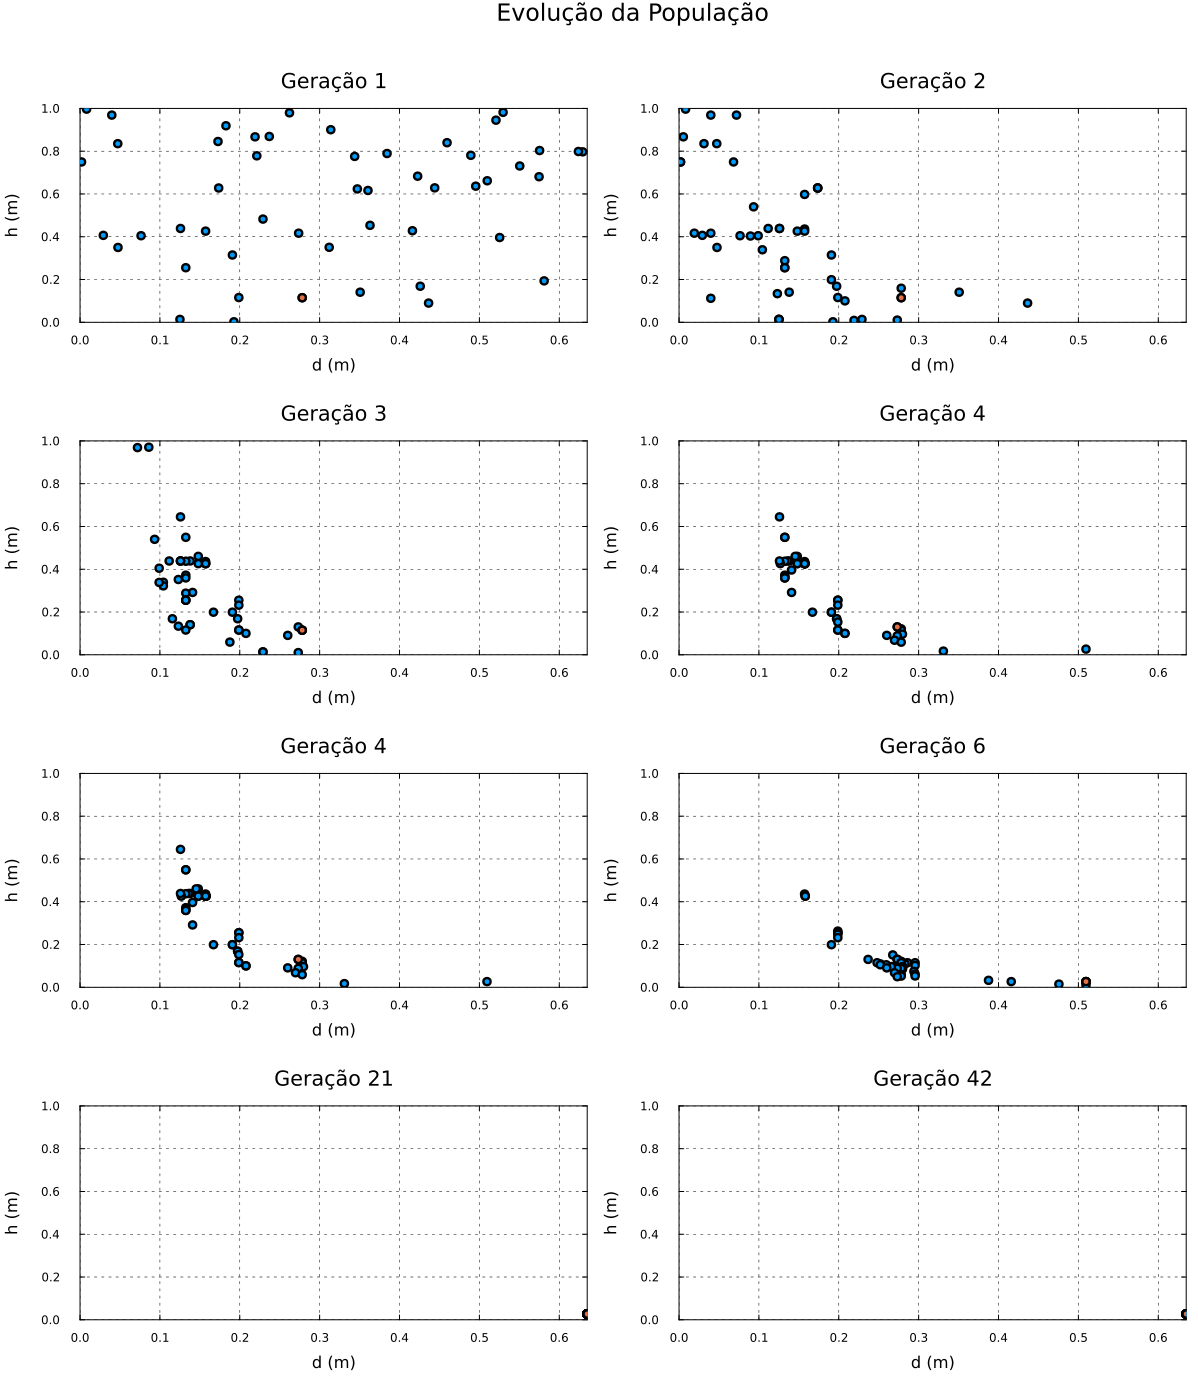
\includegraphics[width=0.9\textwidth]{img/problema_1_populacao.png}
    \caption{Evolução da população do problema 1 de velocidade angular fixa em $3000$ rpm.}
    \label{fig:populacao_1}
\end{figure}

Conforme observado na sequência cronológica da Figura \ref{fig:populacao_1}, a Geração 1 exibe uma distribuição e dispersão uniformes de indivíduos espalhados aleatoriamente por todo o domínio de busca delimitado pelas restrições de caixa. Entre as Gerações 2 e 6, a pressão exercida pela seleção por torneio força uma rápida migração vertical e horizontal. A população abandona as zonas de baixa energia e as zonas proibidas, e então passa a se acumular de forma densa ao longo da curva hiperbólica de restrição ativa de massa. A partir da Geração 21 e consolidando-se na Geração 42, os operadores genéticos provocam o colapso completo da variância populacional, concentrando todos os indivíduos em um único ponto isolado, o qual representa a convergência exata para o ótimo paramétrico global encontrado.

\subsubsection*{Velocidade Angular Variável (Problema II)}

Ao estender o vetor de projeto para incluir a velocidade angular $\omega$ como variável de decisão contínua entre $2000$ e $4000\text{ rpm}$ ($\omega \in [200\pi/3, 400\pi/3]\text{ rad/s}$), a complexidade do problema é ampliada devido ao aumento da dimensionalidade do espaço de busca. A Figura \ref{fig:convergencia_2} registra o comportamento da convergência da energia armazenada máxima ao longo das iterações para o Problema II tridimensional.

\begin{figure}[H]
    \centering
    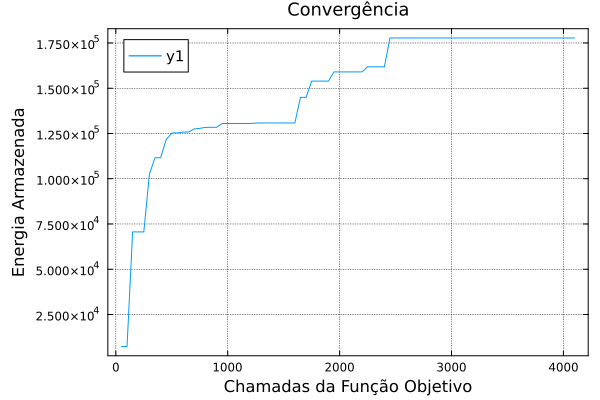
\includegraphics[width=0.6\textwidth]{img/problema_2_convergencia.png}
    \caption{Convergência da função objetivo do problema 2 de velocidade angular variável.}
    \label{fig:convergencia_2}
\end{figure}

Em comparação com o cenário bidimensional, a curva de convergência da Figura \ref{fig:convergencia_2} exige um número visivelmente maior de chamadas à função objetivo para atingir a estabilização assintótica, aproximadamente 4000 chamadas para convergência completa em comparação com as 2000 chamadas do Problema I. Isso ocorre porque o algoritmo precisa sintonizar de forma coordenada três parâmetros acoplados não-linearmente ($d, h, \omega$). Graças ao aumento do índice de distribuição da mutação polinomial para $\eta=10$, as transições entre os degraus de energia tornam-se mais suaves e refinadas, permitindo passos de alta precisão nas proximidades do limite de falha por energia de distorção do aço, atingindo um patamar energético superior próximo a $1,75 \times 10^5\text{ J}$.

A Figura \ref{fig:populacao_2} apresenta a dispersão da população de $N=50$ indivíduos no espaço tridimensional definido pelos eixos coordenados do diâmetro $d$, da altura $h$ e da velocidade angular $\omega$.

\begin{figure}[H]
    \centering
    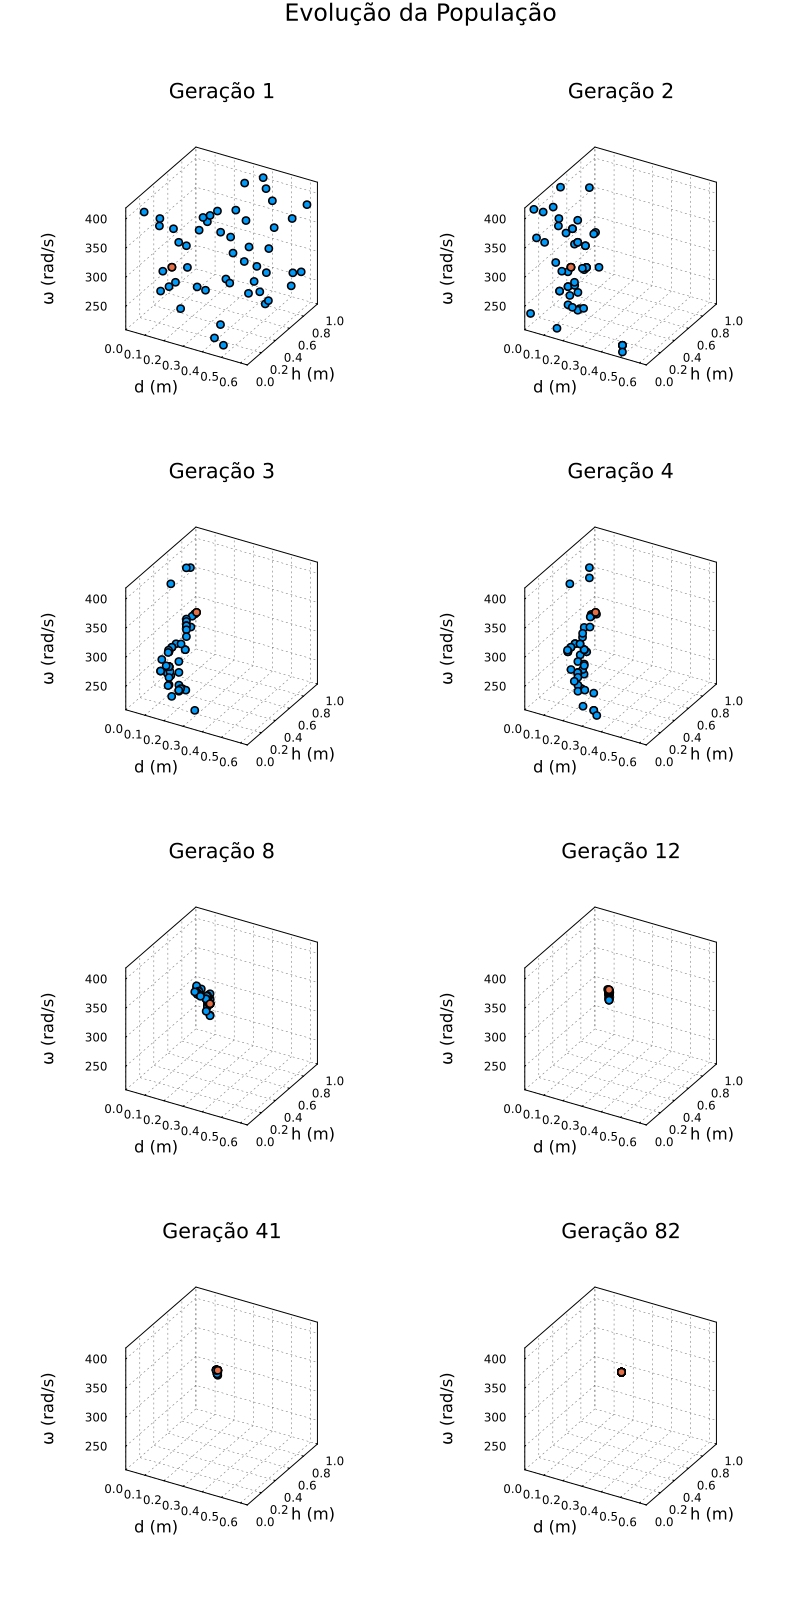
\includegraphics[width=0.7\textwidth]{img/problema_2_populacao.png}
    \caption{Evolução da população do problema 2 de velocidade angular variável.}
    \label{fig:populacao_2}
\end{figure}

A análise volumétrica da Figura \ref{fig:populacao_2} fornece uma prova visual do funcionamento eficiente do algoritmo genético em alta dimensão. Na Geração 1, as partículas ocupam o volume tridimensional de forma esparsa e exploratória. Rapidamente, nas Gerações 2 a 4, a população descarta as regiões proibidas e realiza uma exploração ao longo das diferentes rotações. Nas gerações finais (Gerações 41 a 82), a população condensa-se fortemente em uma coordenada terminal de velocidade e diâmetro.

\subsubsection*{Resultados da Otimização}

Os resultados ótimos encontrados pelo Algoritmo Genético foram compilados estruturadamente. A Tabela~\ref{tab:resultados_otimizacao} apresenta a comparação quantitativa entre o Problema I e o Problema II. Cada variante detalha as dimensões geométricas finais do disco de aço, os parâmetros físicos resultantes e a capacidade total de armazenamento energético do sistema KERS.

\begin{table}[H]
    \centering
    \caption{Comparação dos resultados de otimização paramétrica para os Problemas I e II.}
    \label{tab:resultados_otimizacao}
    \vspace{0.2cm}
    \begin{tabular}{lcc}
        \toprule
        \textbf{Propriedade da Solução} & \textbf{Problema I (Rotação Fixa)} & \textbf{Problema II (Rotação Livre)} \\
        \midrule
        Diâmetro Ótimo ($d$) & $0,6350\text{ m}$ ($635,00\text{ mm}$) & $0,4883\text{ m}$ ($488,30\text{ mm}$) \\
        Altura Ótima ($h$) & $0,0270\text{ m}$ ($27,03\text{ mm}$) & $0,0463\text{ m}$ ($46,35\text{ mm}$) \\
        Velocidade Angular ($\omega$) & $314,16\text{ rad/s}$ ($3000\text{ rpm}$) & $418,88\text{ rad/s}$ ($4000\text{ rpm}$) \\
        Massa Resultante ($m$) & $67,0545\text{ kg}$ & $67,9864\text{ kg}$ \\
        \textit{Massa Limite} & \textit{($68,00\text{ kg}$)} & \textit{($68,00\text{ kg}$)} \\
        Tensão de Pico ($\sigma_{\max}$) & $1,29 \times 10^8\text{ Pa}$ & $1,35 \times 10^8\text{ Pa}$ \\
        \textit{Tensão Limite (Escoamento)} & \textit{($1,38 \times 10^8\text{ Pa}$)} & \textit{($1,38 \times 10^8\text{ Pa}$)} \\
        \textbf{Energia Armazenada ($E$)} & $\mathbf{166.784,30\text{ J}}$ & $\mathbf{177.769,07\text{ J}}$ \\
        \bottomrule
    \end{tabular}
\end{table}

A análise comparativa dos dados revela que a inclusão da velocidade angular como variável de decisão livre no Problema II expandiu a região viável do espaço de projeto, permitindo uma solução superior que resultou em um acréscimo de aproximadamente $6,58\%$ na energia cinética máxima armazenada. No Problema I, o algoritmo foi limitado pelo limite geométrico superior do diâmetro e a única forma de buscar o aumento da inércia de rotação era expandindo o raio até a restrição de tensão, ajustando a espessura para não violar a restrição hiperbólica de massa útil. 

No Problema II, por outro lado, o algoritmo genético maximizou energia utilizando a rotação máxima permitida. Para viabilizar fisicamente essa rotação elevada sem causar a falha por tensão, o otimizador reduziu o diâmetro para $0,4883\text{ m}$ ($23,1\%$ menor que o limite) e compensou a perda volumétrica aumentando a altura do cilindro para $46,35\text{ mm}$. Em ambos os cenários, nota-se que a meta-heurística foi capaz de fazer a população tangenciar com extrema precisão os limites restritivos de projeto, deixando a massa resultante ativa no limiar crítico e a tensão mecânica de pico muito próxima ao escoamento admissível do aço.

\newpage

\subsection*{Questão 6}

O trabalho de controle ótimo escolhido foi o ``Continuous Low-Thrust Maneuver Planning for Space Gravitational Wave Formation Reconfiguration Based on Improved Particle Swarm Optimization Algorithm", publicado em Sensors (2023), desenvolvido por pesquisadores vinculados a institutos de Xangai e da Missão TianQin, incluindo o Laboratório Key do Ministério da Educação para a Missão TianQin, da Universidade Sun Yat-sen.

\subsubsection*{O Problema Abordado e sua Relevância}

O trabalho foca na estratégia de reconfiguração com consumo mínimo de combustível para uma formação tridimensional composta por três satélites arranjados em um triângulo equilátero nominal. A missão está posicionada em uma órbita geocêntrica alta com raio de aproximadamente $100.000$ km, voltada especificamente para a detecção espacial de ondas gravitacionais de baixa e média frequência.

Os métodos tradicionais baseados na medição contínua e direta do estado relativo entre os satélites tornam-se inviáveis ou excessivamente complexos e dispendiosos.

O planejamento das manobras deve garantir precisão nanométrica no posicionamento ao mesmo tempo em que minimiza o tempo de atuação ou queimas de alta frequência dos micropropulsores para evitar perturbações nas massas de teste científicas suspensas no interior dos satélites.


\subsubsection*{Modelo Dinâmico e Hipóteses Simplificadoras}

Para contornar as limitações de medição direta, adota-se o conceito de \textbf{Formação Virtual}. Define-se um ponto de referência matemático operando em uma órbita nominal idealizada, denominado \textit{chief} virtual. Os satélites físicos reais (\textit{deputies}) rastreiam suas respectivas referências de proximidade, descentralizando o problema de controle.

O movimento relativo de cada satélite físico em relação ao seu ponto virtual é descrito pelas equações linearizadas baseadas em Elementos de Órbita Relativa (ROE) quase não-singulares:
\begin{equation}
    \delta\alpha = \begin{pmatrix} \delta a & \delta\lambda & \delta e_x & \delta e_y & \delta i_x & \delta i_y \end{pmatrix}^T
\end{equation}
Onde $\delta a$ representa a diferença normalizada do semieixo maior, $\delta\lambda$ é o argumento médio relativo de longitude, $\delta e$ é o vetor de excentricidade relativa e $\delta i$ é o vetor de inclinação relativa. A dinâmica linearizada perturbada com aceleração de empuxo contínuo é expressa por:
\begin{equation}
    \delta\dot{\alpha}(t) = A(\alpha_c(t)) \begin{bmatrix} \delta\alpha(t) \\ \Delta B_{srp} \end{bmatrix} + \begin{bmatrix} B(\alpha_c(t)) \\ \mathbf{0}_{1 \times 3} \end{bmatrix} u(t)
\end{equation}
Onde $A(\alpha_c(t)) = A_{kep} + A_{J_2}(t) + A_{3rd}(t) + A_{srp}(t)$ representa a matriz completa da planta contendo as superposições do movimento Kepleriano e das forças perturbadoras:
\begin{itemize}
    \item O efeito do achatamento da Terra ($J_2$).
    \item A aceleração perturbadora da Pressão de Radiação Solar (SRP).
    \item A atração gravitacional de terceiro corpo (Sol e Lua).
\end{itemize}

O vetor $u(t) = \begin{bmatrix} u_r & u_t & u_n \end{bmatrix}^T$ define as acelerações de controle nos eixos Radial, Tangencial e Normal (RTN).

\subsubsection*{Hipóteses Simplificadoras}
\begin{itemize}
    \item A órbita de referência do \textit{chief} virtual é considerada quase circular, permitindo ignorar os termos de ordem superior dependentes da excentricidade nas matrizes de perturbação.
    \item A distância de separação mútua entre o satélite físico e a órbita virtual é ordens de magnitude menor do que o raio orbital total ($10^5$ km), validando a aproximação linear.
    \item Fatores dinâmicos secundários, tais como efeitos de sombra/eclipse na radiação solar, gravidade de outros corpos planetários e harmônicos geo-potenciais de alta ordem são explicitamente negligenciados.
    \item As medições osculantes dos satélites são processadas por um filtro numérico de média móvel para extração dos elementos médios, eliminando oscilações transitórias e evitando desperdício de combustível contra efeitos de curto período.
\end{itemize}

\subsubsection*{Critério de Otimização Escolhido}
O objetivo central é formular um controle ótimo de mínimo combustível executado sob um horizonte de tempo finito $t \in [t_0, t_f]$. O problema é categorizado como um Problema de Programação Não Linear Restrita (NLP).

A função objetivo (índice de desempenho $J$) que quantifica o consumo total (Delta-V) da formação é definida por:
\begin{equation}
    \min_{u, t_c} J = \sum_{k_i=1}^{i}(|u_{r,k_i}|+|u_{t,k_i}|)\cdot(t_{i,2k_i}-t_{i,2k_i-1}) + \sum_{k_o=1}^{o}|u_{n,k_o}|(t_{o,2k_o}-t_{o,2k_o-1})
\end{equation}

Sujeito às seguintes restrições:
\begin{align*}
    \text{Restrições de Contorno Terminais:} \quad & \delta\alpha(t_f) = \delta\alpha_{des} \\
    \text{Limites de Amplitude do Empuxo:} \quad & -u_j \le u_j(t) \le u_j \quad (j = i, o) \\
    \text{Restrições Temporais Operacionais:} \quad & t_0 \le t_1 \le t_2 \le \dots \le t_{2k} \le t_f
\end{align*}
Adicionalmente, incluem-se restrições exclusivas onde o empuxo orbital deve ser estritamente nulo ($u(t) = \mathbf{0}$) durante intervalos reservados para calibração e manutenção interna dos instrumentos ópticos.

\subsubsection*{Método de Solução Adotado}
Propõe-se uma estratégia de atuação por \textbf{empuxo constante por partes} (\textit{piecewise constant thrust}). O horizonte temporal total da missão é discretizado em subintervalos fixos em que apenas uma manobra de queima contínua é permitida por partição, eliminando atuações de alta frequência harmônica nas plataformas.

A resolução numérica do NLP é conduzida por meio de um algoritmo modificado de \textbf{Otimização por Enxame de Partículas Melhorado (IPSO)}. As melhorias estruturais implementadas para assegurar a convergência do sistema não linear multivariável incluem:
\begin{enumerate}
    \item \textbf{Função de Penalidade Segmentada Dinâmica:} Adiciona um termo de penalização modificado Deb à função objetivo que varia em função do número de iterações atuais ($i_c$) e do nível de violação das restrições:
    \begin{equation}
        F(x) = f(x) + (i_c\sqrt{i_c}) P(x)
    \end{equation}
    \item \textbf{Mecanismo de Inércia e Aprendizado Adaptativo:} O fator de inércia $W$ e as constantes de aceleração cognitiva e social ($C_1, C_2$) ajustam-se dinamicamente para priorizar a exploração global nas fases iniciais e o refinamento local intenso nas etapas finais de convergência:
    \begin{align}
        W &= (\omega_{max}-\omega_{min})\times \exp\left(-\zeta\times\left(\frac{i_c}{I_{max}}\right)\right)^2 \\
        C_1 &= c_{1,max}-\frac{(c_{1,max}-c_{1,min})\times i_c}{I_{max}} \\
        C_2 &= c_{2,min}+\frac{(c_{2,max}-c_{2,min})\times i_c}{I_{max}}
    \end{align}
    \item \textbf{Operador de Mutação Aleatória:} Introduz-se uma probabilidade de mutação genotípica em variáveis normalizadas para resgatar o enxame de eventuais mínimos locais precoces.
\end{enumerate}

\subsubsection*{Análise dos Resultados Alcançados}
A validação estatística baseada em 20 simulações independentes comprovou a robustez superior do IPSO em relação ao PSO convencional. Nos testes comparativos, o enxame melhorado exibiu diagramas de \textit{boxplot}, apresentados na Figura \ref{fig:boxplot}, significativamente mais estreitos e livres de dispersões anômalas (\textit{outliers}), garantindo alta estabilidade de convergência.

\begin{figure}[H]
    \centering
    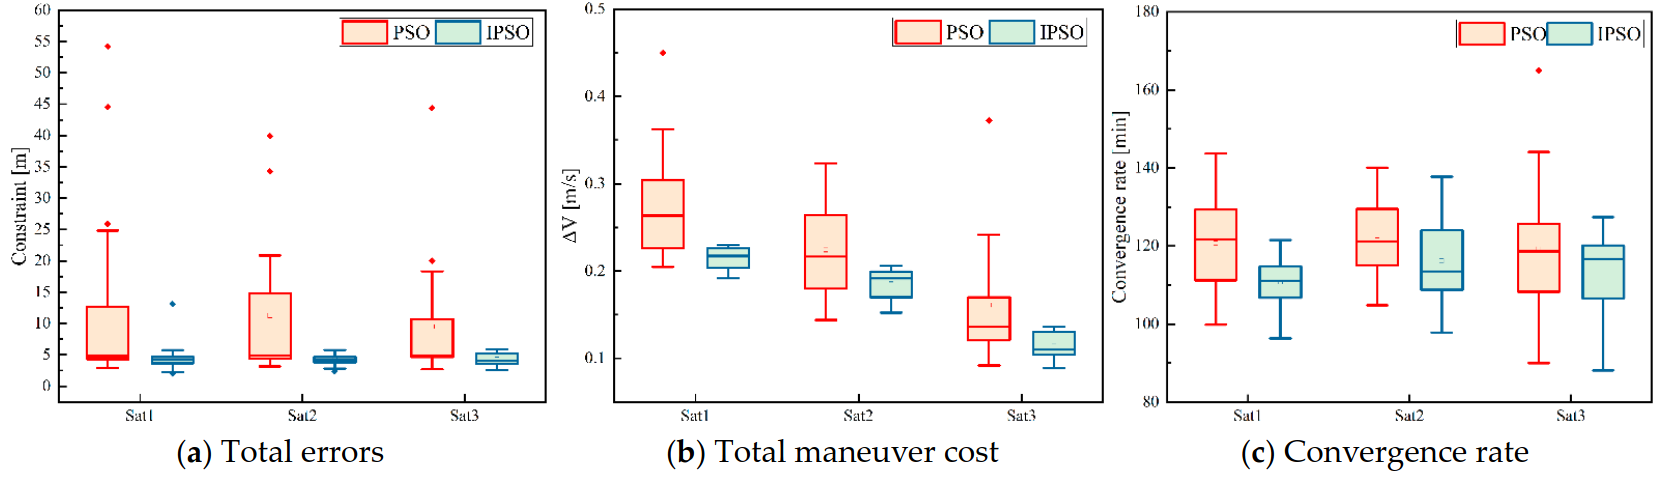
\includegraphics[width=0.8\textwidth]{img/boxplot.png}
    \caption{Comparação estatística entre o PSO convencional e o IPSO proposto. O algoritmo melhorado apresentou convergência mais estável e consistente, com menor dispersão de resultados e ausência de outliers.}
    \label{fig:boxplot}
\end{figure}

\subsubsection*{Otimização e Perfil de Consumo}
Diferentemente dos planejamentos da literatura que focam em queimas unicamente tangenciais, a atuação simultânea nos eixos radial e tangencial mitigou com eficiência o erro acumulado em $\delta\lambda$. Em termos absolutos de consumo de combustível, o algoritmo proposto alcançou valores ótimos de Delta-V inferiores aos métodos contínuos clássicos de mercado reduzindo o custo de um dos satélites de $0,3895$ m/s para $0,2023$ m/s.

\subsubsection*{Uniformidade e Precisão}
Enquanto o método analítico convencional concentrou queimas massivas e instáveis no encerramento da janela temporal para forçar o cumprimento das restrições de contorno, o perfil gerado pelo IPSO distribuiu as acelerações de forma harmônica e estável ao longo de todo o horizonte temporal. 

Por fim, a precisão métrica final de reconfiguração foi validada com extremo sucesso frente aos propagadores orbitais numéricos de alta fidelidade:
\begin{itemize}
    \item O erro máximo de posicionamento relativo terminal não ultrapassou \textbf{3,454 metros}.
    \item O desvio de velocidade relativa terminal manteve-se abaixo de \textbf{3,390 mm/s}.
\end{itemize}
Estes parâmetros atestam que a metodologia de controle ótimo formulada atende perfeitamente aos rigorosos critérios de estabilidade exigidos pelas missões espaciais de detecção de ondas gravitacionais.

\end{document}